\documentclass[aspectratio=169]{beamer}
\usepackage{basileabeam}
\usepackage{epigraph}
\usepackage{graphicx}
\usepackage{multirow}
%\usepackage{enumitem}
\usepackage{array}
%\newcolumntype{C}[1]{>{\centering\arraybackslash}m{#1}}
\newcolumntype{L}[1]{>{\raggedright\let\newline\\\arraybackslash\hspace{0pt}}m{#1}}
\newcolumntype{C}[1]{>{\centering\let\newline\\\arraybackslash\hspace{0pt}}m{#1}}
\newcolumntype{R}[1]{>{\raggedleft\let\newline\\\arraybackslash\hspace{0pt}}m{#1}}

%notes
%\pgfpagesuselayout{2 on 1}[a4paper,border shrink=5mm]
%\setbeamertemplate{note page}[plain]
%\setbeameroption{show notes on second screen=bottom}

\title              {Análise dos modos, efeitos e criticidade de falhas}
\author             {Marco Reis}
\email              {marcoreis@me.com}
\institute          {Laboratório de Robótica e Sistemas Autônomos, Senai Cimatec}
\date               {Abril de 2020}
\ulogo        		{Template/logosenaicimatec}
\ulogoo        		{Template/fibonacci}
\ulistelement    	{Template/sunflower}

\graphicspath{{Figures/}}

\totalNoSlidesDisabled % To turn off the total number of slides in the footer. Comment this if you want the total number of slides in the footer

\begin{document}
%*----------- COVER ------------------------------------------------------------
\begin{frame}[t,plain]
    \titlepage
\end{frame}
%-
\note{Notes can help you to remember important information. Turn on the notes option.}
%*----------- SLIDE ------------------------------------------------------------
\begin{frame}[t]{Introdução} 
%! esta figura tem que sair daqui
A técnica é conhecida como FMECA (\textit{Failure Mode and Effect Criticality Analysis}).

A análise dos modos de falhas, efeitos e criticidade é uma técnica que oferece três funções distintas:
\newline
    \begin{columns}[c]
        \column{.05\textwidth}
        \column{.6\textwidth}
            \begin{enumerate}
                \item ferramenta para prognóstico de problemas
                \item procedimento para desenvolvimento e execução de projetos, processos ou serviços (novos ou revisados)
                \item diário do projeto, processo ou serviço
            \end{enumerate}
        \column{.35\textwidth}
            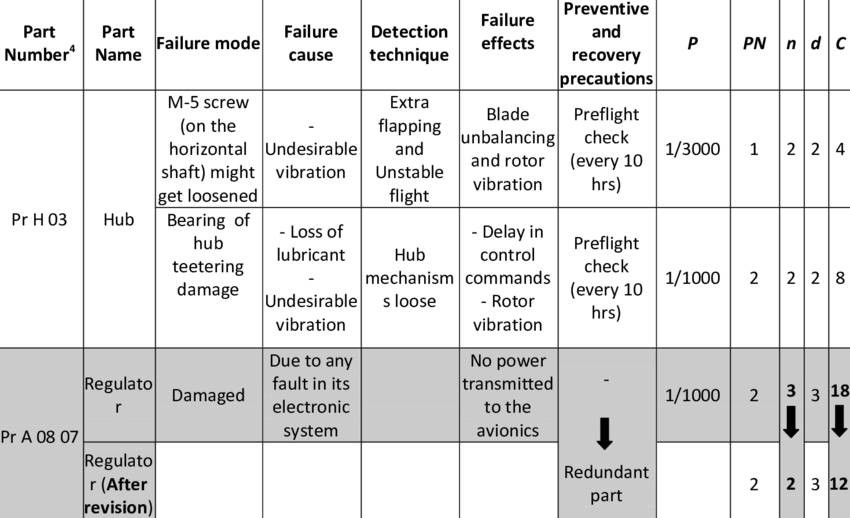
\includegraphics[width=.9\textwidth]{fmeca}
    \end{columns}
\end{frame}
%-
\note{Notes can help you to remember important information. Turn on the notes option.}
%*----------- SLIDE ------------------------------------------------------------
\begin{frame}[t]{FMECA}
    A elaboração da FMECA é muito eficaz quando elaborado em equipe.

    É um método sistemático para identificar e prevenir problemas potenciais.

    Inicialmente, é importante detalhar o sistema em análise apontando os seus subsistemas e componentes.
    
    \setlength\epigraphwidth{.7\textwidth}
    \epigraph{Uma pessoa fazendo o seu melhor, não consegue ser tão eficiente quanto uma equipe trabalhando em conjunto.}{\textit{Marco Reis}}

    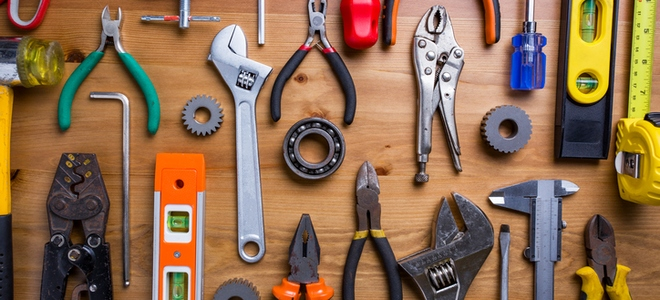
\includegraphics[width=1\textwidth, trim={0 1.8cm 0 0},clip]{tools}
    \raggedleft
\end{frame}
%-
\note{Notes can help you to remember important information. Turn on the notes option.}
%*----------- SLIDE ------------------------------------------------------------
\begin{frame}[t]{Duas Perguntas}
    Quando o foco é o desenvolvimento de um projeto, duas perguntas diretivas devem ser realizadas.
    \newline
    \begin{itemize}
        \item Como esse projeto pode deixar de fazer o que deve fazer?
        \item O que devemos fazer para prevenir essas falhas potenciais de projeto?
    \end{itemize}
    \hfill

    Principais objetivos de uma FMECA:
    \newline
    \begin{columns}[t]
        \column{.45\textwidth}
            detalhar sistemas em subconjuntos\\
            listar possíveis modos de falhas\\
            analisar cada modo de falha, juntamente com suas possíveis causas e sintomas
        \column{.45\textwidth}
            estimar os efeitos de cada modo de falhas\\
            estimar a criticidade de cada efeito\\
            identificar ações para minimizar falhas
    \end{columns}
\end{frame}
%-
\note{Notes can help you to remember important information. Turn on the notes option.}
%*----------- SLIDE ------------------------------------------------------------
\begin{frame}[t]{The Matrix}
    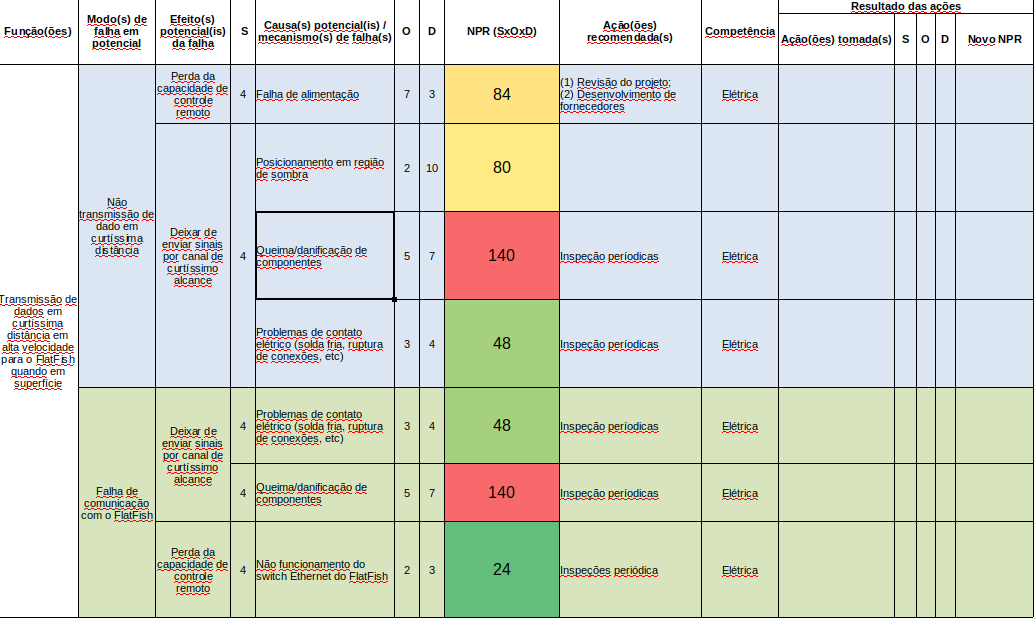
\includegraphics[width=1\textwidth, trim={0 5cm 0 0},clip]{fmeca-matrix}
    %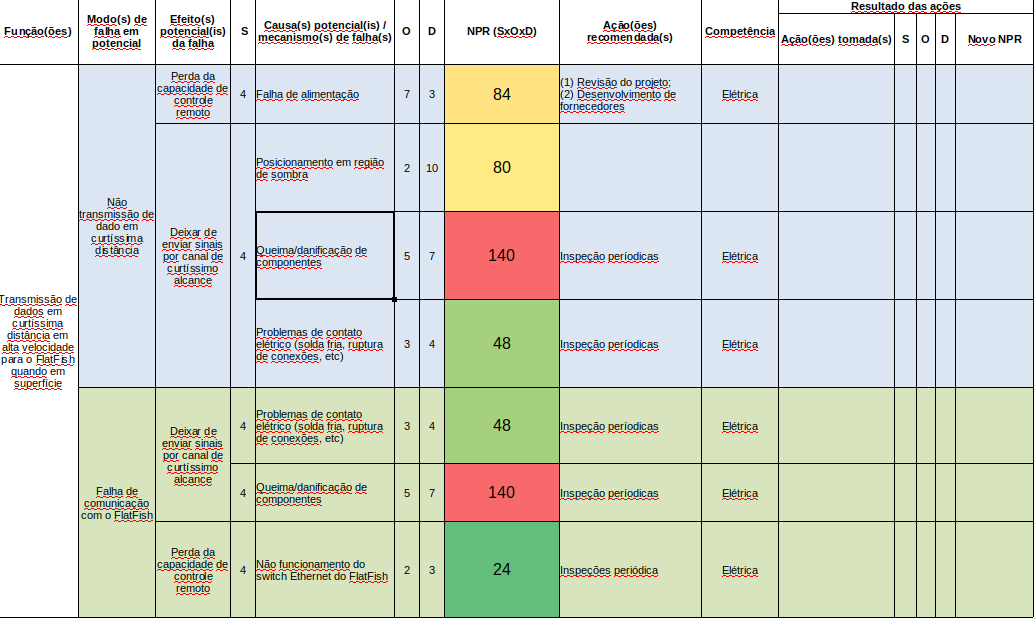
\includegraphics[width=.9\textwidth]{fmeca-matrix}
    \centering
\end{frame}
%-
\note{Notes can help you to remember important information. Turn on the notes option.}
%*----------- SLIDE ------------------------------------------------------------
\begin{frame}[c]{Os padrões}
    \begin{columns}
        \column{.05\textwidth}
        \column{.25\textwidth}
            
\includegraphics[width=1\textwidth, trim={5cm 0 5cm 0},clip]{normas}
        \column{.7\textwidth}
            \begin{itemize}
                \item A FMECA está presente em toda a indústria.
                \item A escalabilidade de cada parâmetro avalaiado apresenta certa diferença entre as áreas aplicadas.
                \item Apesar da variabilidade entre as aplicações nas indústrias, algumas normas são tomadas como referência:
                \begin{itemize}
                    \item SAE standard: J-1739 (automotive systems)
                    \item SAE standard: ARP-5580 (non-automotive systems)
                    \item Military standard: MIL-STD-882
                    \item ESA: ECSS-Q-30-02A
                \end{itemize}
            \end{itemize}
    \end{columns}
\end{frame}
%-
\note{Notes can help you to remember important information. Turn on the notes option.}
%*----------- SLIDE ------------------------------------------------------------
\begin{frame}[t]{Planejando a FMECA}
    \begin{itemize}
            \item O uso da ferramenta busca alcançar o maior potencial de retorno de qualidade e confiabilidade, priorizando sempre os pontos mais críticos.
            \item Deve-se restringir o uso para conjuntos e subconjuntos e, somente em alguns casos extender para componentes.
            \item Quando necessário, quebrar as funções do sistema para que os conjuntos ou subconjuntos possam ser analisados.
    \end{itemize}
    \vspace{1cm}
    \hspace*{0.5cm}\emph{Como pode falhar? Porque falha? O que acontece quando falha?}
%
\end{frame}
%-
\note{Notes can help you to remember important information. Turn on the notes option.}
%*----------- SLIDE ------------------------------------------------------------
\begin{frame}[t]{Regras básicas}
    \begin{itemize}
            \item A construção e a análise da FMEA exigem a utilização de outras ferramentas de suporte à qualidade e confiabilidade. Geralmente, os dados devem ser analisados utilizando-se métodos estatísticos antes de preencher uma das colunas da FMEA ou aprovar as recomendações para medidas corretivas.
            \item Não considerar todos os modos de falha concebíveis. Isso aumenta o custo e a duração da análise, sem nenhum benefício real.
            \item Redigir o modo de falha como expressão negativa da função.
            \item Selecionar uma abordagem para classificar os modos e causas de falhas, ou seja classificação das ocorrências e detecção das causas.
            \item Desenvolver independentemente cada coluna da matriz FMECA.
            \item Um pré-requisito para o FMECA é a definição de todas as exigências das várias especificações e a garantia de que todos os membros da equipe adquiram um nível de compreensão funcional dessa especificações.
    \end{itemize}
\end{frame}
%-
\note{Notes can help you to remember important information. Turn on the notes option.}
%*----------- SLIDE ------------------------------------------------------------
\begin{frame}[t]{Especificações}
    Há quatro especificações que precisam ser compreendidas e satisfeitas:
    \vspace{.2cm}
    \begin{description}%[lefttmargin=2em,style=nextline]
        \item[Especificações de Engenharia] \hfill \\ incluem exigências funcionais, físicas, dimensionais e químicas.
        \item[Especificações de Confiabilidade] \hfill \\ concentram-se nas exigências de engenharia que operam em vários ambientes e durante períodos específicos.
        \item[Especificações de Qualidade] \hfill \\ concentram-se nas técnicas usadas para projetar e monitorar a qualidade.
        \item[Especificações do Cliente] \hfill \\ refletem o que os clientes querem e esperam do projeto.
    \end{description}
\end{frame}
%-
\note{Notes can help you to remember important information. Turn on the notes option.}
%*----------- SLIDE ------------------------------------------------------------
\begin{frame}[t]{Exemplos}
    \begin{description}%[lefttmargin=2em,style=nextline]
        \item[Especificações de Engenharia] \hfill \\ um sensor para atuar, deve ter seu atuador à distância especificada; um motor não pode ser colocado a funcionar com uma carga mecânica além daquela que foi especificada em projeto.
        \item[Especificações de Confiabilidade] \hfill \\ um componente elétrico para atingir sua vida útil máxima deve ter seu índice de proteção maximizada.
        \item[Especificações de Qualidade] \hfill \\ parâmetros de solda, posicionamento das peças nos dispositivos.
        \item[Especificações do Cliente] \hfill \\ máxima disponibilidade dos equipamentos na linha produtiva; baixo índice de retrabalho nos veículos produzidos; ciclo de produção alcançado ou extrapolado.
    \end{description}
\end{frame}
%-
\note{Notes can help you to remember important information. Turn on the notes option.}
%*----------- SLIDE ------------------------------------------------------------
\begin{frame}[t]{Terminologia}
    \begin{columns}
        \column{.01\textwidth}
        \column{.1\textwidth}
            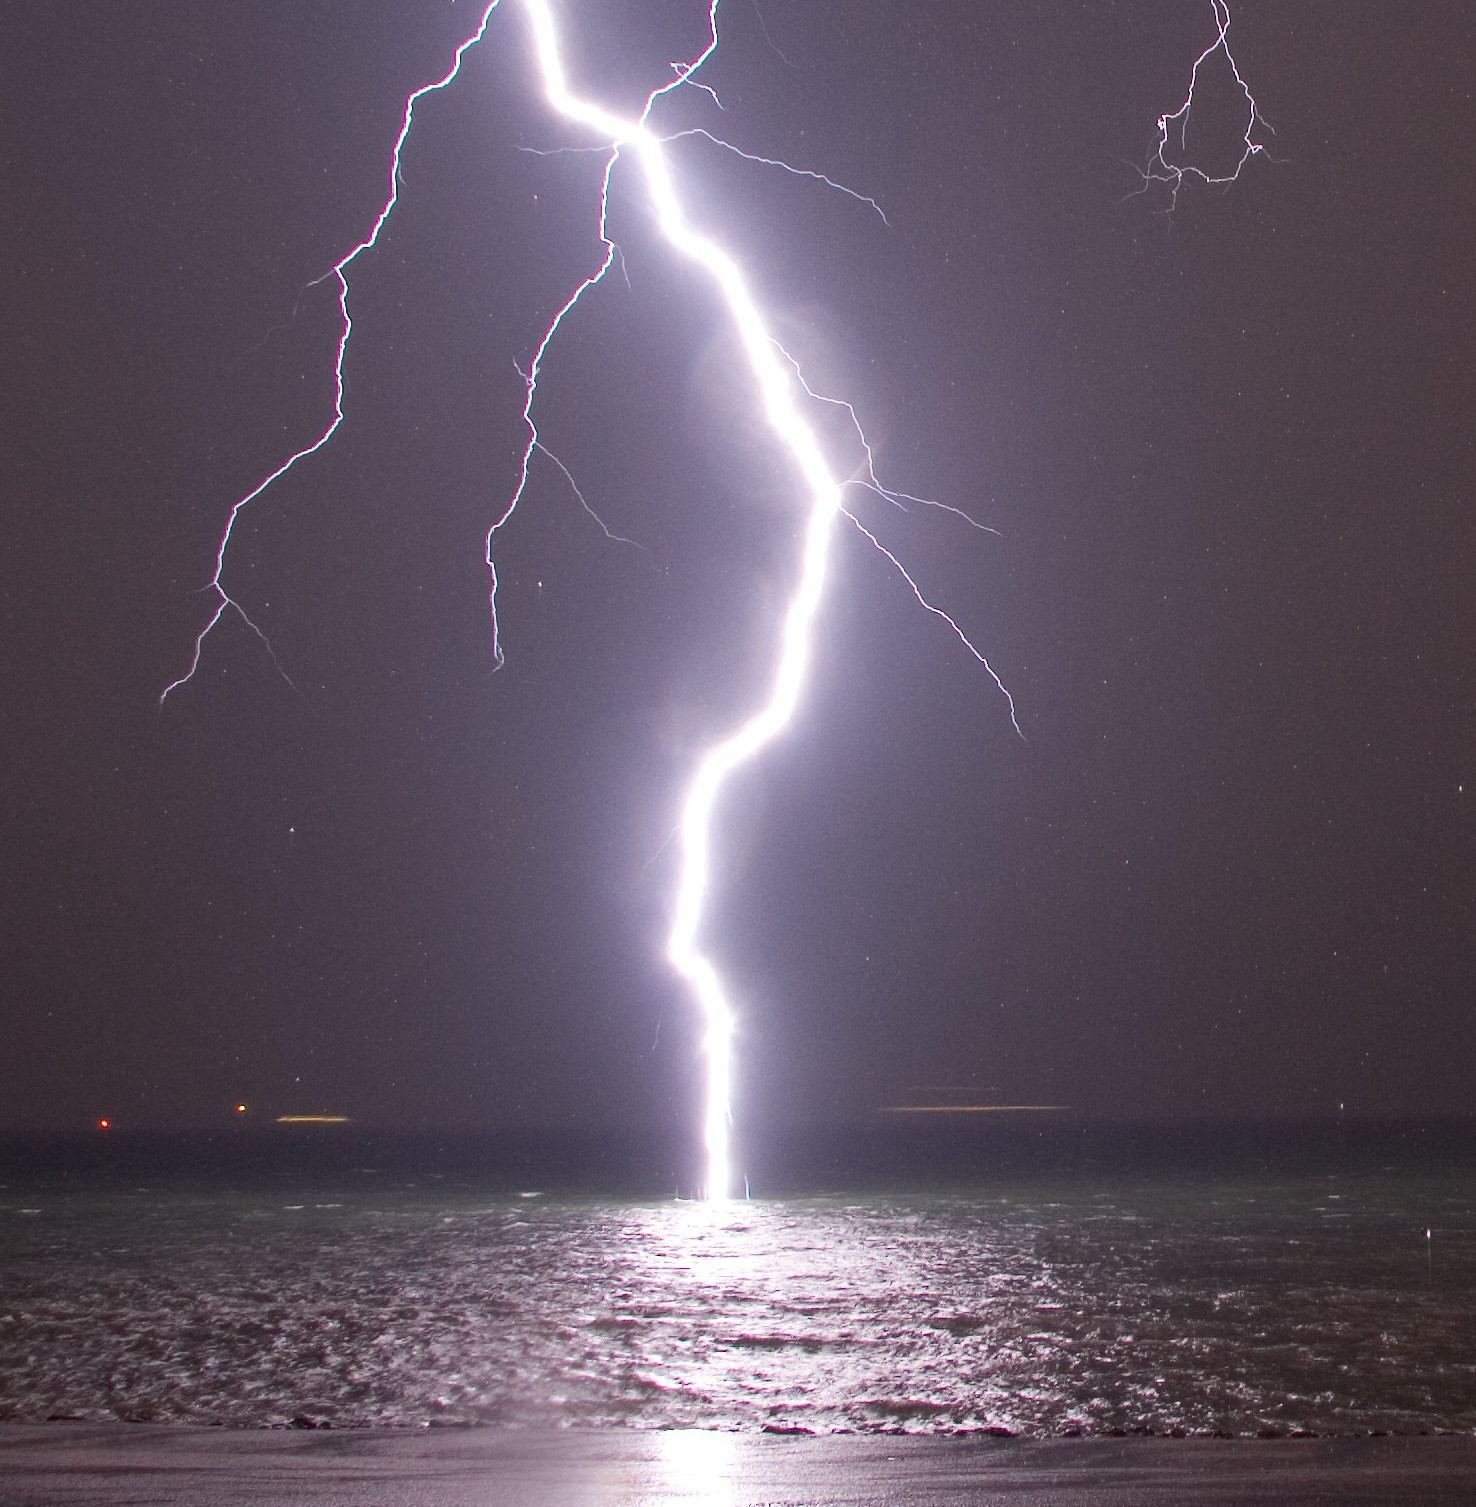
\includegraphics[width=2.2\textwidth, trim={15cm 2cm 15cm 5cm},clip]{raios}
        \column{.9\textwidth}
        \begin{description}[rightmargin=2em,style=nextline]
            \item[FALHA]é qualquer não-conformidade no produto
            \item[MODO DE FALHA] é a não-conformidade que o cliente percebe; considerar dois principais modos: o de não funcionamento e o de funcionamento incorreto dos conjuntos e subconjuntos.
            \item[EFEITO DA FALHA] é a consequência da falha para o cliente; um sintoma de falha indica o modo como uma falha irá se tornar evidente, estes sintomas podem se tornar evidentes tanto antes como após a falha realmente ocorrer. 
            \item[CAUSA DA FALHA] é a causa fundamental da falha; identificar e listar somente as causas principais de cada modo.
        \end{description}
    \end{columns}
\end{frame}
%-
\note{Notes can help you to remember important information. Turn on the notes option.}
%*----------- SLIDE ------------------------------------------------------------
\begin{frame}[t]{Avaliação da FMECA}

    \begin{description}%[rightmargin=2em,style=nextline]
        \item[CRITICIDADE]é o índice de importância para priorizar os modos de falha.
    \end{description}
    \vspace{0.2cm}
    Este índice faz parte da avaliação do FMECA, o mesmo dá-se mediante o cálculo dos índices de Severidade, Ocorrência e Deteção.
    \vspace{0.2cm}

    A Criticidade pode ser chamada também de Risco Prioritário, onde representa a gravidade resultante do cálculo mencionaddo acima.
    \vspace{0.2cm}

    \begin{equation}
    \label{eq:criticidade}
        C = \beta . \lambda . \alpha
    \end{equation}

    \begin{itemize}
        \item $C$ é a criticidade da falha, ou seja o número de prioridade do risco da falha.
        \item $\beta$ é a extensão dos problemas causados pela falha (severidade).
        \item $\lambda$ é a probabilidade estimada da falha ocorrer (ocorrência).
        \item $\alpha$ é a probabilidade estimada da falha ser percebida (detecção).
    \end{itemize}
\end{frame}
%-
\note{Notes can help you to remember important information. Turn on the notes option.}
%*----------- SLIDE ------------------------------------------------------------
\begin{frame}[t]{Severidade}
    O índice de \textbf{Severidade} adotado para o desenvolvimento de projetos da área de robótica considera 10 níveis para o escalonamento.

    Para a avaliação do índice não deve ser considerado somente o efeito localizado mas também os efeitos secundários.
     \begin{columns}
         \column{.2\textwidth}
             
\includegraphics[width=1\textwidth, trim={0 0 0 0},clip]{alerta}
            \column{.8\textwidth}
            \begin{table}[ht]
            \centering
             \resizebox{\textwidth}{!}{%
                \begin{tabular}{|>{\centering\arraybackslash}m{1.5cm}|l|l|}
                    \hline
                    \textbf{valor} & \textbf{Severidade} & \textbf{Critério} \\ \hline
                    1 & Mínima & O cliente mal percebe que a falha ocorre. \\ \hline
                    2 & \multirow{2}{*}{Pequena} & \multirow{2}{*}{Ligeira deteriorização no desempenho com leve descontentamento do cliente.} \\ \cline{1-1}
                    3 &  &  \\ \hline
                    4 & \multirow{3}{*}{Moderada} & \multirow{3}{*}{Deteriorização significativa do desempenho de um sistema com descontentamento do cliente.} \\ \cline{1-1}
                    5 &  &  \\ \cline{1-1}
                    6 &  &  \\ \hline
                    7 & \multirow{2}{*}{Alta} & \multirow{2}{*}{Sistema deixa de funcionar. É grande o descontentamento do cliente.} \\ \cline{1-1}
                    8 &  &  \\ \hline
                    9 & \multirow{2}{*}{Muito alta} & \multirow{2}{*}{Sistema deixa de funcionar. É grande o descontentamento do cliente, porém  afeta a segurança e o ambiente.} \\ \cline{1-1}
                    10 &  &  \\ \hline
                \end{tabular}%
            }
            \end{table}
    \end{columns}
\end{frame}
%-
\note{Notes can help you to remember important information. Turn on the notes option.}
%*----------- SLIDE ------------------------------------------------------------
\begin{frame}[t]{Ocorrência}
    O índice de \textbf{Ocorrência} adotado para o desenvolvimento de projetos da área de robótica considera 10 níveis para o escalonamento.

    Na falta de dados para calcular a probabilidade, os profissionais podem usar da experiência para determinar as frequências típicas para as várias causas de falha e classificá-las de acordo com a sua probabilidade de ocorrência.

    \begin{table}[]
        \centering
        \resizebox{.35\textwidth}{!}{%
        \begin{tabular}{|>{\centering\arraybackslash}m{1.5cm}|l|l|}
        \hline
        \textbf{valor} & \textbf{Ocorrência} & \textbf{Critério} \\ \hline
        1 & Remota & 1:1.000.000 \\ \hline
        2 & \multirow{2}{*}{Pequena} & 1:20.000 \\ \cline{1-1} \cline{3-3}
        3 &  & 1:4.000  \\ \hline
        4 & \multirow{3}{*}{Moderada} & 1:1.000 \\ \cline{1-1} \cline{3-3}
        5 &  & 1:400  \\ \cline{1-1} \cline{3-3}
        6 &  & 1:100 \\ \hline
        7 & \multirow{2}{*}{Alta} & 1:40 \\ \cline{1-1} \cline{3-3}
        8 &  & 1:20 \\ \hline
        9 & \multirow{2}{*}{Muito alta} & 1:8 \\ \cline{1-1} \cline{3-3}
        10 &  & 1:2 \\ \hline
        \end{tabular}%
        }
    \end{table}

\end{frame}
%-
\note{Notes can help you to remember important information. Turn on the notes option.}
%*----------- SLIDE ------------------------------------------------------------
\begin{frame}[t]{Detecção}
    O índice de \textbf{Detecção} adotado para o desenvolvimento de projetos da área de robótica considera 10 níveis para o escalonamento. Este índice deve refletir não somente se os sinais de uma falha iminente são detectáveis, mas também se estes sinais fornecem um tempo de detecção prévia.

    Se uma falha se torna detectável um pouco antes de ocorrer, ela é mais difícil de prevenir do que falhas que apresentam tempos maiores de detecção prévia.

    \begin{table}[ht]
        \centering
        \resizebox{0.5\textwidth}{!}{%
        \begin{tabular}{|>{\centering\arraybackslash}m{1.5cm}|l|l|}
        \hline
        \textbf{valor} & \textbf{Detecção} & \textbf{Critério} \\ \hline
        1 & \multirow{2}{*}{Muito grande} & \multirow{2}{*}{Certamente será detectado.} \\
        2 &  &  \\ \cline{1-1} \cline{2-2} \cline{3-3}
        3 &  \multirow{2}{*}{Grande} & \multirow{2}{*}{Grande probabilidade de ser detectado.} \\ \cline{1-1}
        4 &  &  \\ \cline{1-1} \cline{2-2} \cline{3-3}
        5 &  \multirow{2}{*}{Moderada} & \multirow{2}{*}{Provavelmente será detectado.} \\ \cline{1-1}
        6 &  &  \\ \hline
        7 & \multirow{2}{*}{Pequena} & \multirow{2}{*}{Provavelmente não será detectado.} \\ \cline{1-1}
        8 &  &  \\ \hline
        9 & \multirow{2}{*}{Muito pequena} & \multirow{2}{*}{Certamente não será detectado.} \\ \cline{1-1}
        10 &  &  \\ \hline
        \end{tabular}%
        }
        \end{table}

\end{frame}
%-
\note{Notes can help you to remember important information. Turn on the notes option.}
%*----------- SLIDE ------------------------------------------------------------
\begin{frame}[t]{A construção da matriz}
    Uma demonstração de construção de uma análise
    \vspace{0.5cm}
    \begin{table}[ht]
        \centering
        \resizebox{\textwidth}{!}{%
        \begin{tabular}{|m{2.5cm}|>{\raggedright\arraybackslash}m{3.0cm}|>{\raggedright\arraybackslash}m{3.5cm}|m{1em}|>{\centering\arraybackslash}m{3.5cm}|m{1em}|m{1em}|m{1em}|>{\centering\arraybackslash}m{3.0cm}|}
        \hline
        \multicolumn{1}{|l|}{\textbf{Função}} & \textbf{Modos de falhas em potencial} & \textbf{Efeitos potenciais da falha} & \textbf{S} & \textbf{Causas potenciais de falhas} & \textbf{O} & \textbf{D} & \textbf{C} & \textbf{Ações recomendadas} \\ \hline
        \multirow{3}{7em}{Transmissão de dados em curtíssima distância em alta velocidade para o sistema quando em superfície} & Não transmissão de dado em curtíssima distância & Perda da capacidade de controle remoto & 4 & Falha de alimentação & 7 & 3 & 84 & Revisão do projeto e desenvolvimento de fornecedores \\ \cline{2-9} 
         & \multirow{2}{7em}{Falha de comunicação com o sistema} & Deixar de enviar sinais por canal de curtíssimo alcance & 4 & Problemas de contato elétrico (solda fria, ruptura de conexões, etc) & 3 & 4 & 48 & Inspeção períodicas \\ \cline{3-9} 
         &  & Perda da capacidade de controle remoto & 3 & Queima/danificação de componentes & 5 & 7 & 105 & Inspeção períodicas \\ \hline
        \end{tabular}%
        }
    \end{table}
    
\includegraphics[width=1\textwidth, trim={0 4.5cm 0 4.5cm},clip]{trabalho}
\end{frame}
%-
\note{Notes can help you to remember important information. Turn on the notes option.}
%*----------- SLIDE ------------------------------------------------------------
\begin{frame}[t]{Como preencher a matriz}
    \begin{description}[rightmargin=2em,style=nextline]
        \item [Função:] Deve-se identificar todas as funções do sistema. Uma forma de analisar é identificar as entradas da funcionalidade.
        \item [Modos de falhas em potencial:] Listar de que forma as entradas listadas podem falhar, ou seja, como essas entradas poderão não desempenhar suas funções. Lembrar que a pergunta chave é: Como pode falhar?
        \item [Efeitos potenciais da falha:] Deverão ser descritos as conseqüências de cada um dos módulos de falha. 
        \item [Severidade:] A pergunta chave deste ponto é ”Qual a gravidade das consequencias dos efeitos anteriores que resultam dos modos de falhas?” A medida de severidade baseia-se em custos e segurança, e estas têm de ser as premissas.
    \end{description}
\end{frame}
%-
\note{Notes can help you to remember important information. Turn on the notes option.}
%*----------- SLIDE ------------------------------------------------------------
\begin{frame}[t]{Como preencher a matriz}
    \begin{description}[rightmargin=2em,style=nextline]
        \item [Causas potenciais de falhas:] Identifica todas as razões que podem resultar na ocorrência do modo de falha. Lembre-se que muitos eventos podem contribuir para um modo de falha; entretanto , como sugere o principio de Pareto, muitas dessas causas contribuem pouquíssimo e apenas algumas contribuem realmente, as ”causas básicas”, e devem ser identificadas no FMECA.
        \item [Ocorrência:] O que essa coluna pergunta é: ”Com que freqüência o modo de falha ou causa tende a ocorrer?”. Devemos levar em conta o histórico de falhas para classificar essa coluna.
        \item [Detecção:] Define o nível de detecção da falha antes que ela ocorra, ou seja, antes que ela apareça.
    \end{description}
\end{frame}
%-
\note{Notes can help you to remember important information. Turn on the notes option.}
%*----------- SLIDE ------------------------------------------------------------
\begin{frame}[t]{Como preencher a matriz}
    \begin{description}[rightmargin=2em,style=nextline]
        \item [Criticidade:] Esta coluna realiza a multiplicação da Severidade, Ocorrência e Detecção. Quanto maior o valor numérico, maior a criticidade. A escala adotada depende da decisão da equipe que elabora a FMECA, objetivando sempre separar as falhas potenciais do restante. 
        \item [Ações recomendadas:] Devem ser eficazes em termos de custos e devem ter um alto grau de permanência. Envolve desde a revisão do da funcionalidade, até a revisão do projeto, fato que deverá evidenciado através de um estudo.
    \end{description}
\end{frame}
%-
\note{Notes can help you to remember important information. Turn on the notes option.}
%*----------- SLIDE ------------------------------------------------------------
\begin{frame}[t]{Observações importantes}
    \begin{itemize}
        \item uma única causa pode ser a origem de diferentes tipos de falha;
        \item um único problema pode ser gerado pro diferentes causas;
        \item a consequência é sempre o impacto da falha no cliente;
        \item lembrar sempmre o princípio de Pareto:\footnote{afirma que para muitos eventos, aproximadamente 80\% dos efeitos vêm de 20\% das causas} poucos vitais e muitos triviais;
        \item as relações de causa e efeito podem ser complexas. 
    \end{itemize}
    \vspace{0.2cm}
    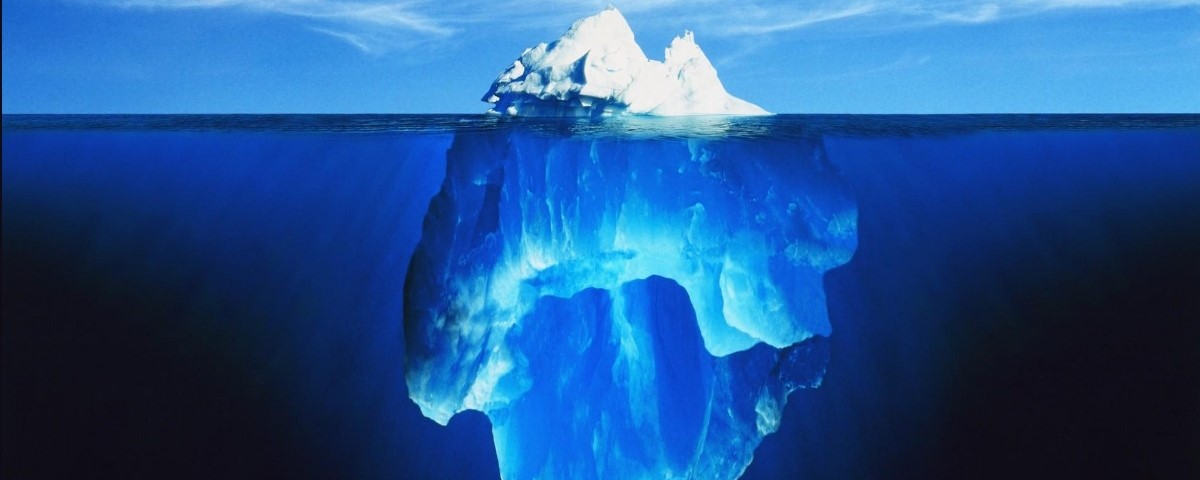
\includegraphics[width=1\textwidth, trim={0 6cm 0 0},clip]{iceberg}
\end{frame}
%-
\note{Notes can help you to remember important information. Turn on the notes option.}
%*----------- SLIDE ------------------------------------------------------------
\begin{frame}[c]{Exemplo}
    Pela manhã, você vai ligar seu carro e percebe que ele não dá nem sinal de partida.
    \vspace{.5cm}
    \begin{columns}[c]
        \column{0.5\textwidth}
            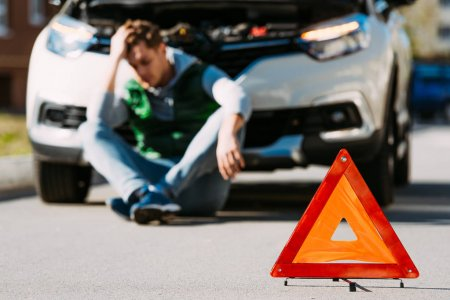
\includegraphics[width=0.6\textwidth, trim={0 0 0 0},clip]{carro-quebrado}
            \centering
        \column{0.5\textwidth}
            \emph{O que seria a causa,\\o modo da falha \\e o efeito da falha?}
    \end{columns}
    \vspace{.5cm}
    \begin{description}[rightmargin=1em,style=nextline]
        \item[MODO] carro não pega, não dá sinal de partida
        \item[EFEITO] chegar atrasado no trabalho, gastar dinheiro com o conserto do carro 
        \item[CAUSA] falta de gasolina, problema elétrico ou problema mecânico
    \end{description}
\end{frame}
%-
\note{Notes can help you to remember important information. Turn on the notes option.}
%*----------- SLIDE ------------------------------------------------------------
% \begin{frame}[c]{Speaker Notes}
% You may turn on the notes and handout option to see the notes to the slides.
% \end{frame}
% %-
% \note{Notes can help you to remember important information. Turn on the notes option.}
%*----------- BACKUP -----------------------------------------------------------
\backupbegin
%*----------- SLIDE ------------------------------------------------------------
\begin{frame}[t]{Backup}
Test
\end{frame}
%-
\note{Notes can help you to remember important information. Turn on the notes option.}
%
\backupend
%*----------- QUESTIONS --------------------------------------------------------
\begin{frame}[t,plain]
\lastpage{{\usebeamerfont{title} Questions?}\\[3ex] \hspace{0.1cm} marcoreis@me.com}
\end{frame}
%-
\note{Notes can help you to remember important information. Turn on the notes option.}
%*--------------------------------------------------------------------- END-----
\end{document}